
\documentclass[11pts,a4paper,amsmath,amssymb,floatfix]{article}
\usepackage{graphicx}% Include figure files
\usepackage{enumerate}% Align table columns on decimal point
\usepackage{bm,dpfloat}% bold math
\usepackage{amsfonts,amsthm,amsmath,amssymb,stmaryrd,indentfirst}
\usepackage{times,psfrag,pdfpages}
\usepackage{framed,comment,lscape}
\usepackage{float,cancel}

\newcommand{\frc}{\displaystyle\frac} 
\newcommand{\eg}{{\it e.g., }}
\newcommand{\ie}{{\it i.e., }}
\newcommand{\wrt}{{\it wrt }}
\newcommand{\Partial}[3][error]{\left(\frc{\partial #1}{\partial #2}\right)_{#3}}
\newcommand{\mfr}[3][error]{#1_{#2}^{\left(#3\right)}} 
\newcommand{\summation}[3][error]{\sum\limits_{#2}^{#3}#1}

\begin{document}
\begin{center}
 {\bf UNIT CONVERSION FACTORS}
\end{center}

%%% SECTION
\section{Length}\label{Chapter:UnitConversion:Section:Length}
     \begin{center}
     \begin{tabular}{|l l l l l|}
       \hline
       1 m =& 3.2808 ft =& 39.37 in =& 10$^{2}$ cm =& 10$^{10}$ A \\
       1 mm =& 10$^{-3}$ m =& 10$^{-1}$ cm =& 10$^{-6}$ km &       \\
       1 mile =& 5280 ft =& 1609.36 m =& 1.609 km &             \\
       \hline           
     \end{tabular}
     \end{center}
          
%%% SECTION
\section{Area}\label{Chapter:UnitConversion:Section:Area}
     \begin{center}
     \begin{tabular}{|l l l l l|}
       \hline
       1 m$^{2}$ =& 10$^{4}$ cm$^{2}$ =& 10.76 ft$^{2}$ =& 1550 in$^{2}$ & \\
       1 in$^{2}$ =& 6.944$\times$10$^{-3}$ ft$^{2}$ =& 6.4516$\times$10$^{-4}$ m$^{2}$ & & \\
       \hline           
     \end{tabular}
     \end{center}
          
%%% SECTION
\section{Volume}\label{Chapter:UnitConversion:Section:Volume}
     \begin{center}
     \begin{tabular}{|l l l l l|}
       \hline    
       1 m$^{3}$ =& 35.313 ft$^{3}$ =& 6.1023$\times$10$^{4}$ in$^{2}$ =& 1000 l =& 264.171 gal \\
       \hline            
     \end{tabular}
     \end{center}
          
%%% SECTION
\section{Mass}\label{Chapter:UnitConversion:Section:Mass}
     \begin{center}
     \begin{tabular}{|l l l l l|}
       \hline    
        1 kg =& 1000 g =& 2.2046 lbm & & \\
       \hline            
     \end{tabular}
     \end{center}


          
%%% SECTION
\section{Force}\label{Chapter:UnitConversion:Section:Force}
     \begin{center}
     \begin{tabular}{|l l l l l|}
       \hline    
         1 N =& 10$^{5}$ dyne =& 1 kg.m.s$^{-2}$ =& 0.225 lbf & \\
       \hline            
     \end{tabular}
     \end{center}

     
%%% SECTION
\section{Energy}\label{Chapter:UnitConversion:Section:Energy}
     \begin{center}
     \begin{tabular}{|l l l l l|}
       \hline
       1 J =& 1 N.m  =& 1 kg.m$^{2}$.s$^{-2}$ =& 9.479$\times$10$^{-4}$ Btu &  \\
       1 kJ =&  1000 J  =&  0.9479 Btu  =& 238.9 cal &                      \\
       \hline           
     \end{tabular}
     \end{center}
     
%%% SECTION
\section{Power}\label{Chapter:UnitConversion:Section:Power}
     \begin{center}
     \begin{tabular}{|l l l l l|}
       \hline
       1 W =& 1 J.s$^{-1}$  =& 1 kg.m$^{2}$.s$^{-3}$ =& 3.412 Btu.h$^{-1}$ =& 1.3405$\times$10$^{-3}$ hp   \\
       1 kW =&  1000 W  =& 3412 Btu.h$^{-1}$  =& 737.3 ft.lbf.s$^{-1}$ =& 1.3405 hp  \\
       \hline           
     \end{tabular}
     \end{center}
     
%%% SECTION
\section{Pressure}\label{Chapter:UnitConversion:Section:Pressure}
     \begin{center}
     \begin{tabular}{|l l l l l|}
       \hline
       1 Pa =& 1 N.m$^{-2}$ =& 1 kg.m$^{-1}$.s$^{-2}$ =& 1.4504$\times$10$^{-4}$ lbf.in$^{-2}$ & \\
       1 atm =& 14.696 lbf.in$^{-2}$ =& 1.01325$\times$10$^{5}$ Pa =& 101.325 kPa =& 760 mm-Hg \\
       1 dyne.cm$^{-2}$ =& 0.1 Pa =& 10$^{-6}$ bar =& 145.04 lbf.in$^{-2}$ & \\
       1 bar =& 10$^{5}$ Pa =& 0.987 atm =& 14.504 lbf.in$^{-2}$ & \\
       \hline           
     \end{tabular}
     \end{center}
     
%%% SECTION
     \section{Temperature}\label{Chapter:UnitConversion:Section:Temperature}
     \begin{displaymath}
       \begin{cases}
         T\left(^{\circ}F\right) = \frc{9}{5}T\left(^{\circ}C\right) + 32 = T(R) - 459.67 & \\
         T\left(^{\circ}C\right) = \frc{5}{9}\left[T\left(^{\circ}F\right)-32\right] = T(K) - 273.15 & 
       \end{cases}      
     \end{displaymath}
     
%%% SECTION
     \section{Viscosty}\label{Chapter:UnitConversion:Section:Viscosity}
     \begin{center}
     \begin{tabular}{|l l l l l|}
       \hline
       1 Pa.s =& 1 N.s.m$^{-2}$ =& 1 kg.m$^{-1}$.s$^{-1}$ =& 10 poise &   \\
       1 poise =& 1 dyne.s.cm$^{-2}$ =& 1 g.cm$^{-1}$.s$^{-1}$ =& 0.1 Pa.s =& 6.72$\times$10$^{-2}$ lbm.ft$^{-1}$.s$^{-1}$\\
       1 stoke =& 1 cm$^{2}$.s$^{-1}$ =& 10$^{-4}$cm$^{2}$.s$^{-1}$ =& 1.076$\times$10$^{-3}$ ft$^{2}$.s$^{-1}$ & \\
       \hline           
     \end{tabular}
     \end{center}
     


 
%%%
%%% 
  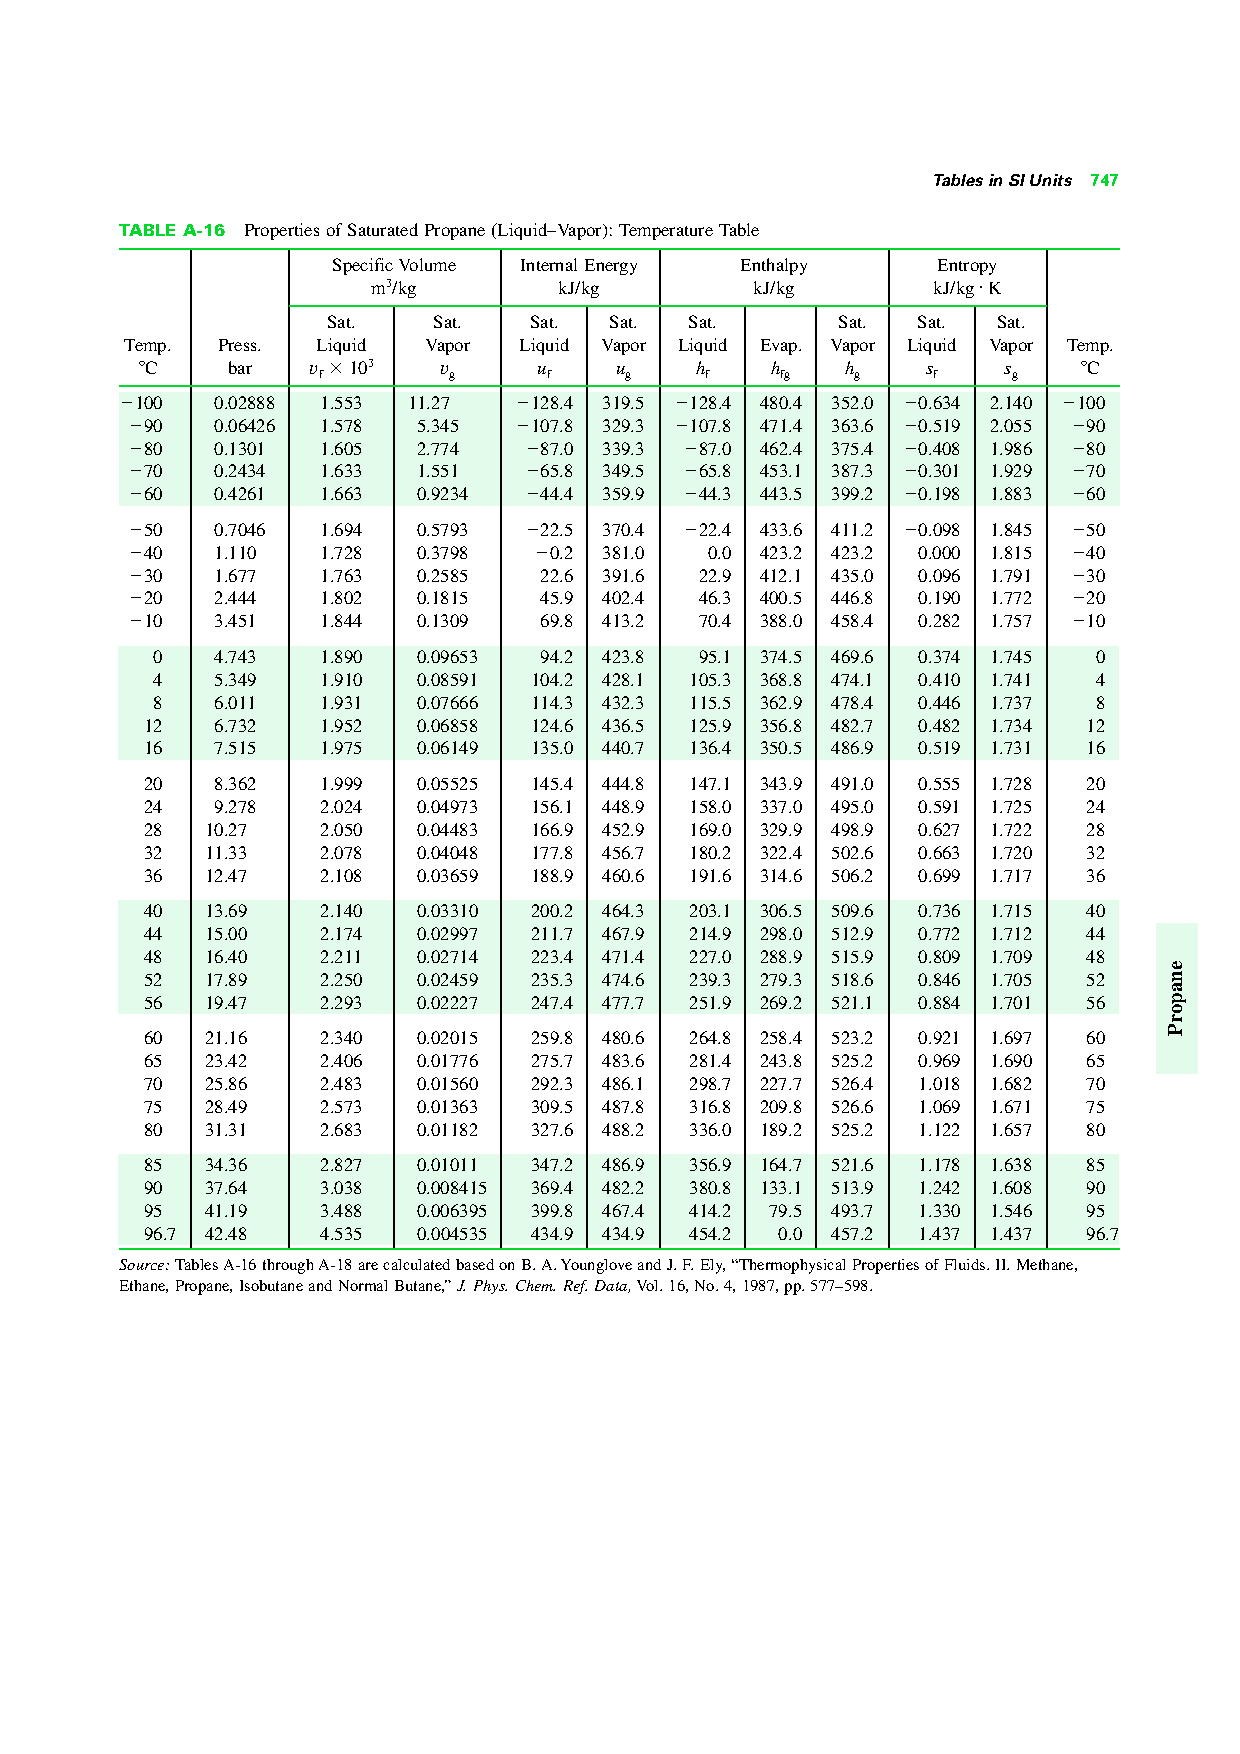
\includepdf[scale=1,pages=-,pagecommand={}, fitpaper]{./Tables/SatProp_Propane.pdf} 


\end{document}
